\chapter{Background Studies}
\label{chap:back}

\textit{The decay \Bmumumu is a fully leptonic decay with good potential for eliminating many types of the backgrounds. In this chapter parametrisation and estimations for all considered backgrounds are sketched. A quick summary of all backgrounds that past the stringent selection were provided in~\autoref{bkgquick}.}


\section{Combinatorial Background}
Combinatorial background comes around as a random combination of tracks from different $b$-decay chains.  The usual method at \gls{LHCb} of estimating the amount and the shape of this background include extrapolation from the upper mass data sideband to the signal region. In this case the upper mass sideband is defined as $M_{\rm{B_{corr}}} > 5500 \mevcc$ and the signal region is defined to be $ 4500 \mevcc <M_{\rm{B_{corr}}} < 5500 \mevcc$. The characteristic shape for this background can be described by exponential function up to certain point, where this point is the primary discusion of this section. Since tight selection resulted in low-statistics data samples the extrapolation from upper mass sideband introduces a big uncertainty on the exponential constant and cannot be used to estimate the correct shape and yield of this background. What can be done, however, is to assume the exponential shape for combinatorial component and let the exponential constant be a floating parameter in the data fit. This method for estimation of the combinatorial component will be re-explained in data mass fits\mybox{SALLY:maybe reference}. In the rest of this section exponential parametrisation of this background between $4000 \mevcc <M_{\rm{B_{corr}}} < 7000 \mevcc$ is motivated. This is important as the final fitting region was chosen in such a way as to make sure that combinatorial background is exponential in this entire fitting region. 

Apart from the nominal upper mass data sideband sample, two other samples are analysed as proxies for this type of background. Despite the fact that these samples are also scarcely populated they are studied altogether to determine in which mass regions the combinatorial background can be considered exponential. Firstly, same sign data sample was studies (the same one as in~\autoref{cloniatkos}), where this sample consists of $\mu^{+} \mu^{+} \mu^{+} \nu$ events passing all selection up to MVA selection to have sufficient statistics. Secondly an inclusive $b\bar{b}$ simulation sample consisting of events where two muons with $p > 3$ \gevc are required to be present together with a third muon that hae passed through all the stripping selection. This exponential component stops rising at low $M_{\rm{B_{corr}}}$ in all samples. As seen in~\autoref{fig:bbarcombi}(a)(c), the drop appears at $M_{\rm{B_{corr}}} = 4000 \mevcc$. Hence the choice of fitting region $4000 \mevcc<M_{\rm{B_{corr}}}<7000\mevcc$.

\begin{figure}[H]
\center
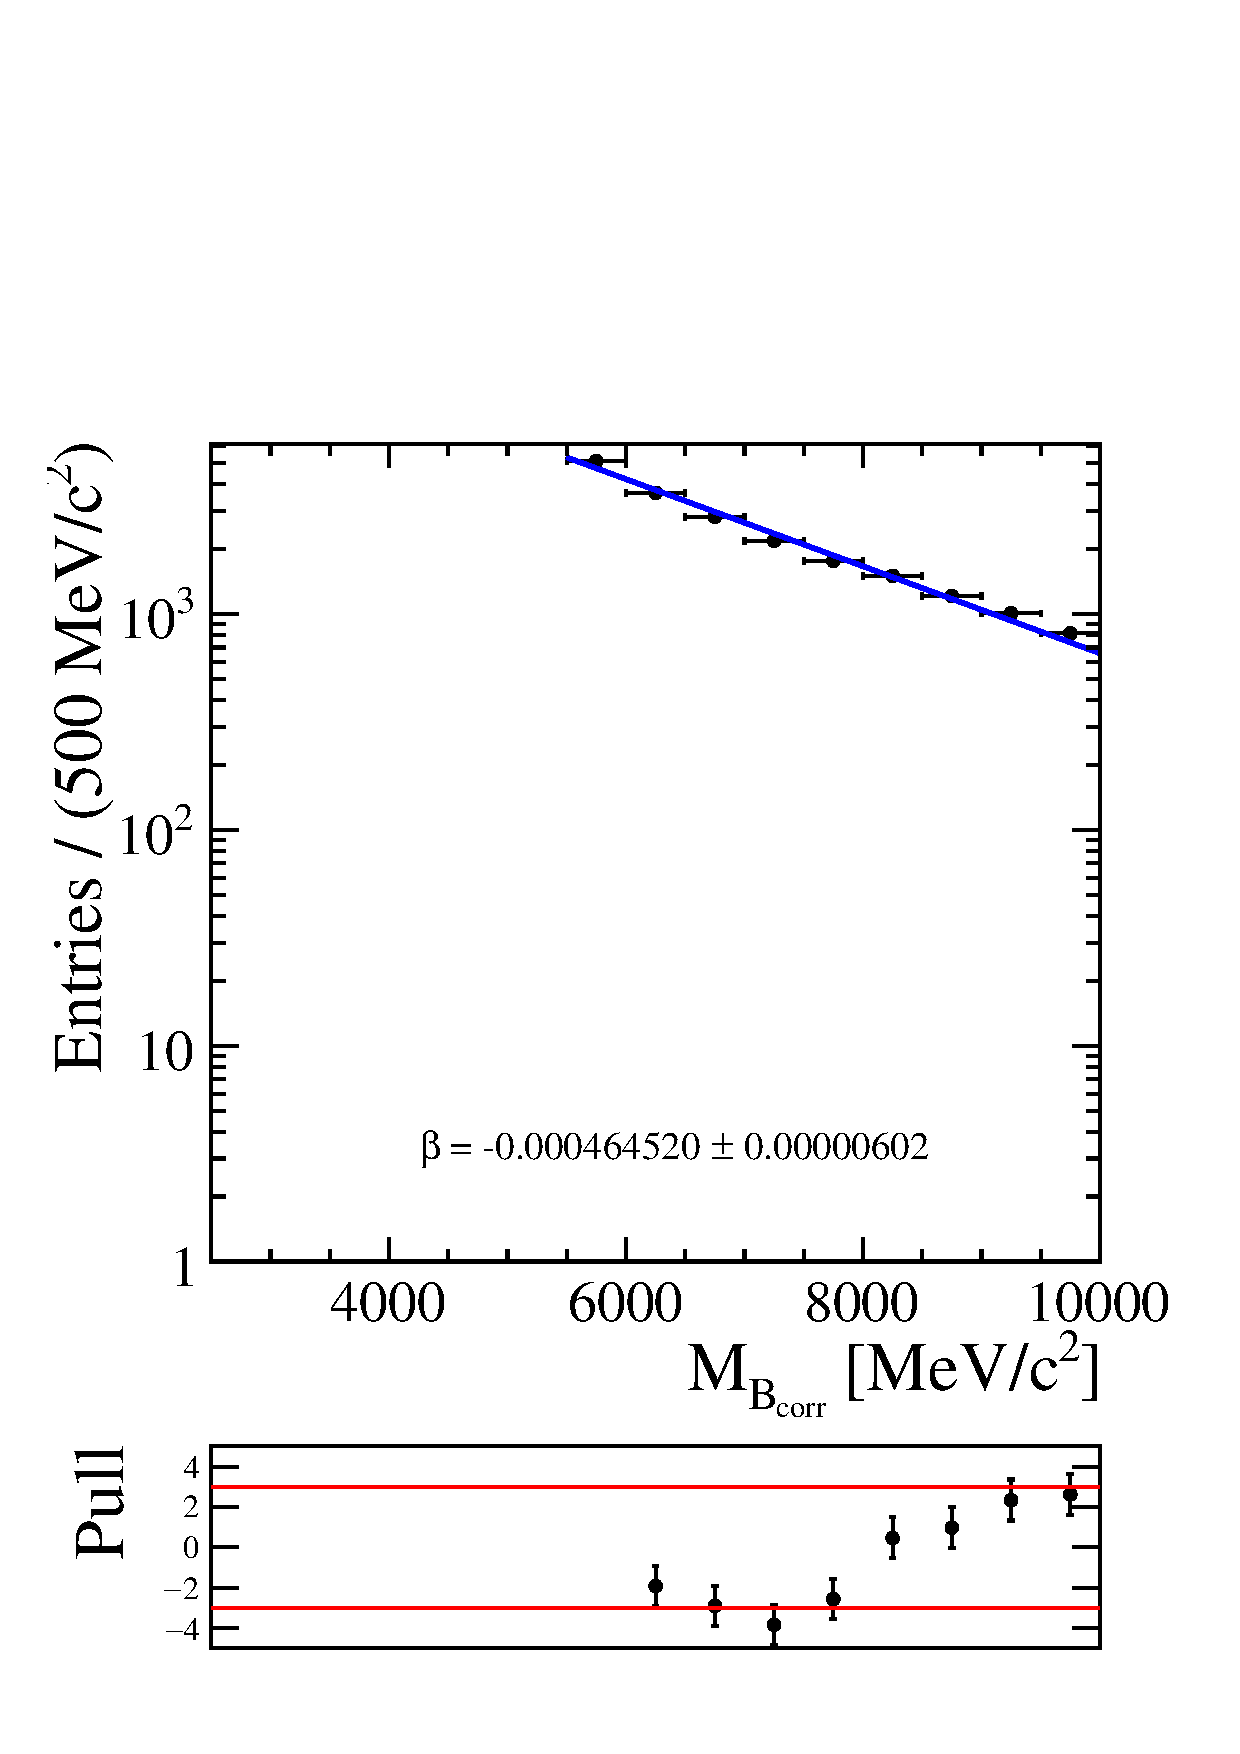
\includegraphics[width = 0.33\textwidth]{bkg/combi/nicenewANAcombiUMSB_WITHPULL_new.pdf}\put(-70,100){(a)}%
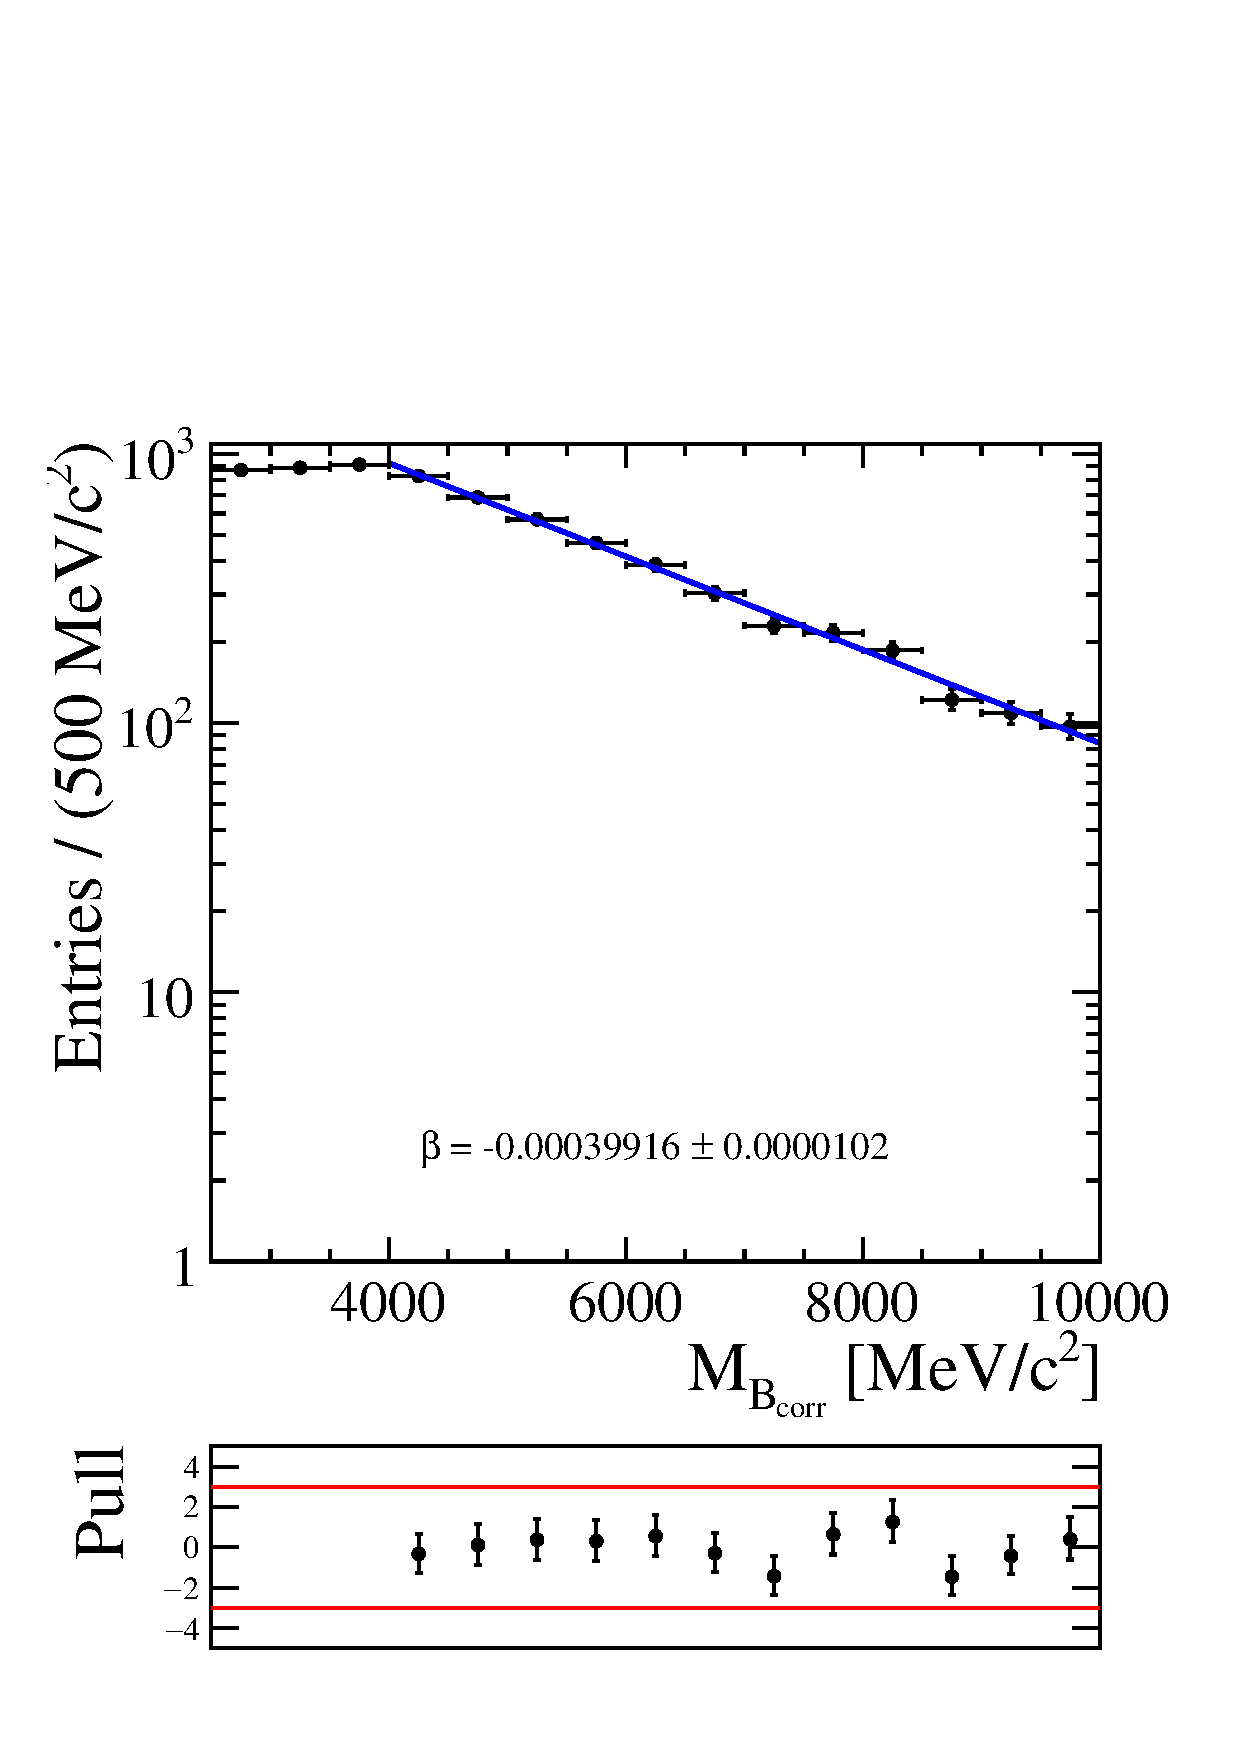
\includegraphics[width = 0.33\textwidth]{bkg/combi/nicenewANAcombi3same_WITHPULL_new.pdf}\put(-70,100){(b)}%
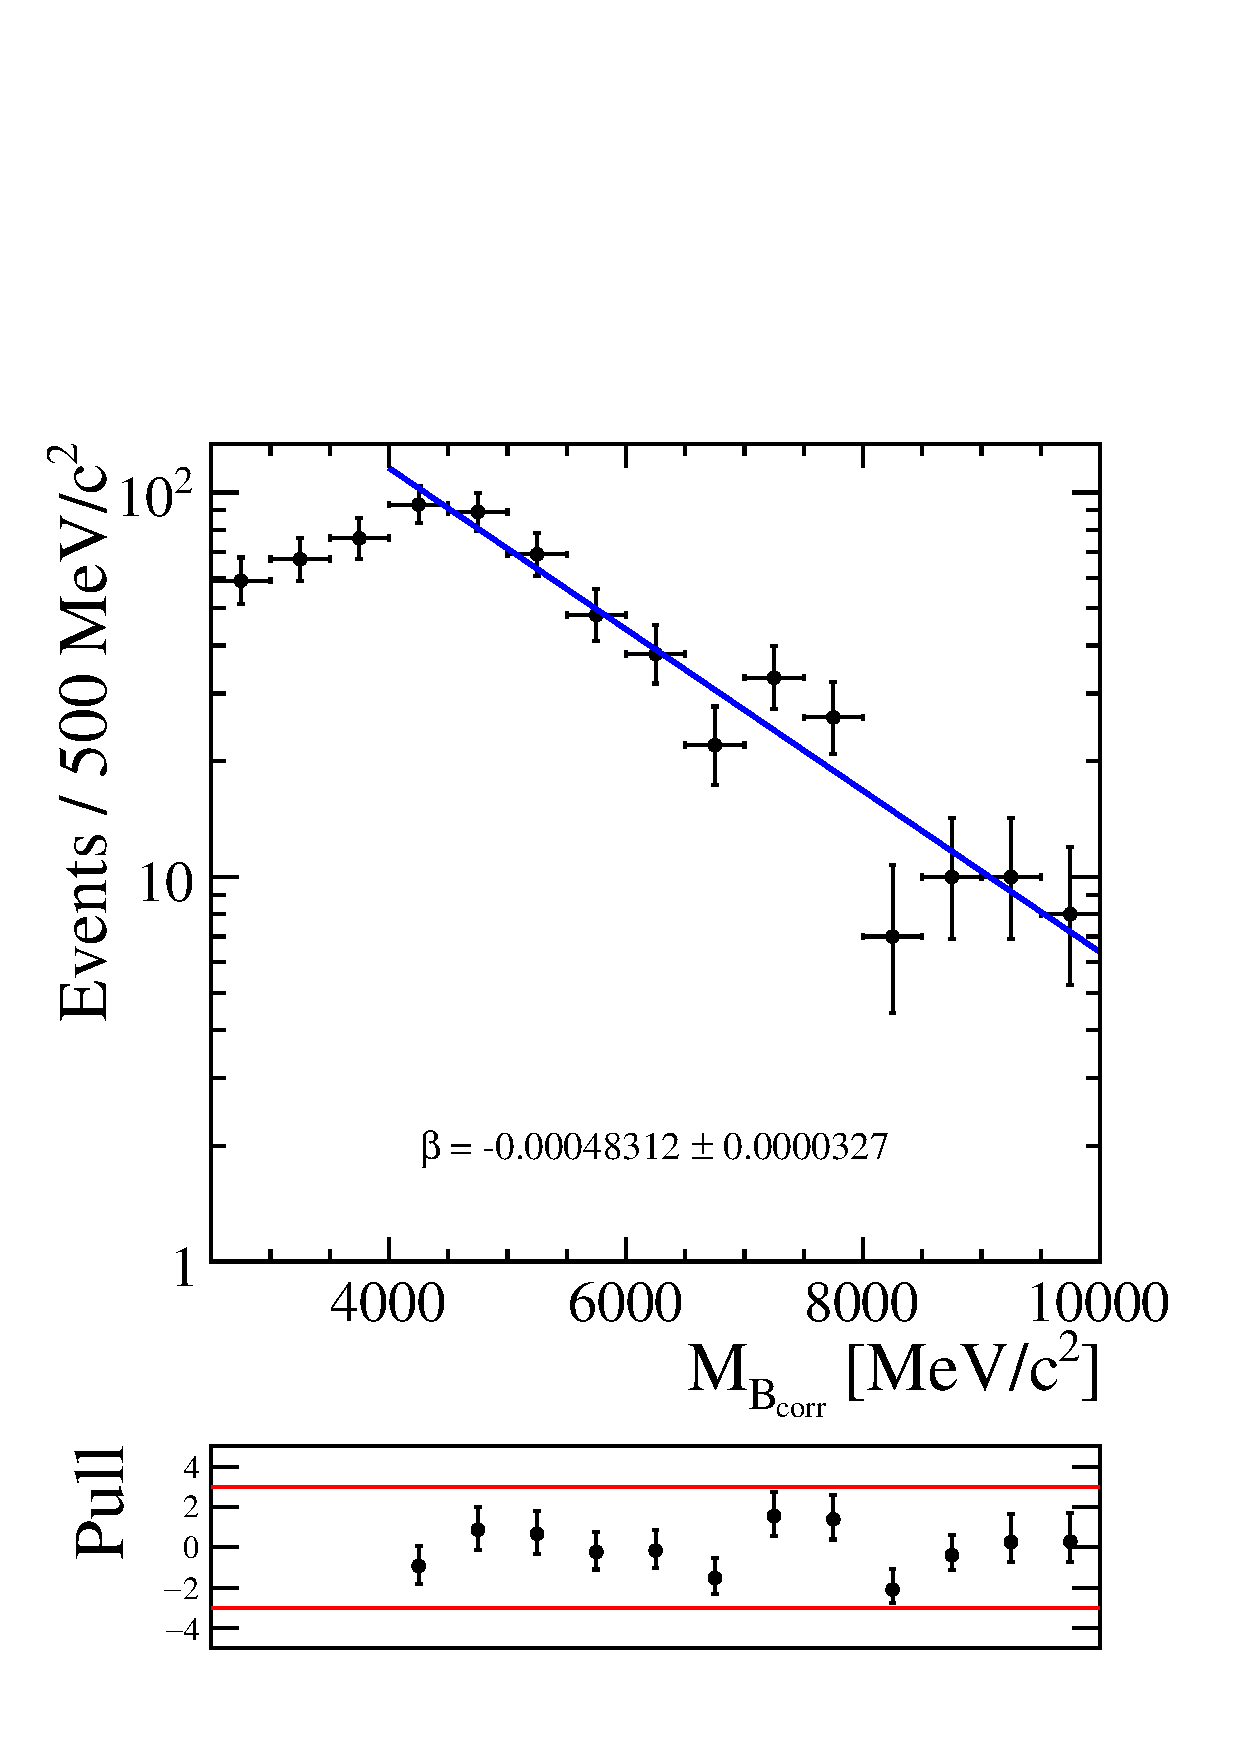
\includegraphics[width = 0.33\textwidth]{bkg/combi/nicenewANAcombi_WITHPULL_new.pdf}\put(-70,100){(c)}%
\caption{(a) Fit to upper mass side band just before application of MVA selection. (b) Fit to $\mu^{+}\mu^{+}\mu^{+}\nu$ same sign sample. (c) Fit to $b\bar{b}$ sample with exponential function. In all examples exponential description is not correct below $4000 \mevcc$.}
\label{fig:bbarcombi}
\end{figure}

This background is heavily supressed with dedicated MVA selection described in~\autoref{CombiBDTsel}.


\subsection{MisID type background}
\label{misidprocedure}
MisID background is one of the most prominent backgrounds that is expected to be present. This type of background proceeds mostly via cascade decays, where $B^{+} \rightarrow (\overline{D^{0}} \rightarrow h X \mu^{-} \nu) \mu^{+} \nu$ and then $h\in[K^{+},\pi^{+}]$ are misidentified as muons. The contributions from decays where two muons are correctly identified as muons and third track is consistent with proton passing all the selection is also considered, however it will be shown that this contribution is very limited. 

As discussed in~\autoref{bkgquick} there are two possibilites for the charge for the misidentified background. In one case the sign of the misidentified particle agrees with the sign of the mother $B$, \textit{SS misID} background. The opposite case is denoted as \textit{OS misID} decays. These two types of backgrounds are studied using data-driven method described below. Finally, also double misID employing same data-driven methods was studied, where there are two hadrons misidentfied as muons, however, the double misID contribution proved to be insignificant.


To determine the amount and the shape of the misID background, data sample with the same selection as for the signal sample is obtained with one marginal difference - \textbf{no \gls{PID} cut} on one muon, either positive or negative. As the muon misID rate is different for pions and kaons~\cite{LHCb-DP-2013-001}, the species of the hadron, $h$ must be determined at first. The strategy for this purpose is to isolate the hadron into separate hadron \gls{PID} regions, and to determine the cross-feed of one region into the other. For this, an iterative procedure as shown in \autoref{fig:misidproc} is applied. It splits the misidentified data sample into three \gls{PID} regions, where the hadron candidate is consistent with the kaon, pion and proton hypotheses. For this procedure, probabilities of identifying a given species with given \gls{PID} requirement are taken from dedicated control samples in data. The \gls{PID} performance is highly dependant on kinematic properties of the misidentified particle and hence the estimation is performed in bins of momentum $p$ and pseudorapidity $\eta$.
At the beginning of the procedure, the number of misidentified events of given species is assumed to be zero, and the
cross-feed between regions is calculated assuming that the pion, kaon and protons regions are pure pions, kaons and protons.
This procedure then corrects the distributions by taking into the account this initial cross-contamination.
This procedure is repeated until the number of total misidentified particles does not change significantly from one iteration to another.

\begin{figure}[h]
  \begin{center}
    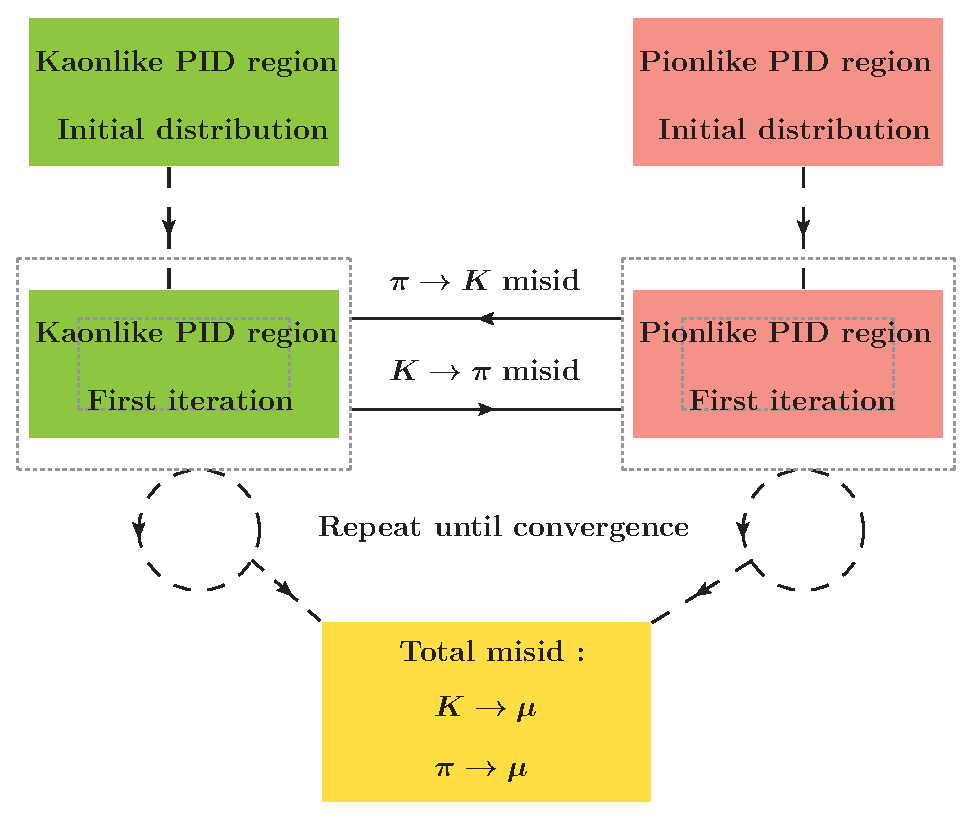
\includegraphics[width=0.6\linewidth]{bkg/misid/misid_att_3}%\put(-32,133){(a)}
    \vspace*{-0.5cm}
  \end{center}
  \caption{
    Diagram of the iterative procedure to establish contamination from decays where pion and kaon are misidentified for muon.
    }
  \label{fig:misidproc}
\end{figure}



Once the cross-feed between the different hadron species has been taken into account, the final step is to calculate the probability for
a specific hadron to pass the stringent muon \gls{PID} requirements applied in the analysis. The presence of the two real muons in the $\mumu h X$
background increases probability to misidentify the hadron as a muon, mainly due to sharing of hits in the muon stations. Therefore the hadron misID probability is obtained from a dedicated control sample designed to emulate the topology of the mis-identified background,
 $B^{0} \rightarrow J/\psi(\rightarrow \mu^{+} \mu^{-}) K^{*}(\rightarrow \underline{K^{+} \pi^{-}})$, as shown in~\autoref{ratiatkos}.

%To determine the amount and the shape of the misID background data sample, same selection as for the signal sample is applied apart from \texttt{no \gls{PID} cut} on one muon, either positive or negative. The stripping selection for this sample is similar but with \texttt{no \gls{PID} cut} for the misidentified muon (SS or OS), see~\autoref{tab:misidbackground}.

This process can be summarized mathematically in a following way:

\begin {itemize}
\item The proton-, pion- and kaon-like regions are defined in~\autoref{tab:misidregions}.

\begin{table}[ht]
\begin{center}
\begin{tabular}[t]{| l | l |}
\hline
Region & PID cuts  \\ \hline
Proton-like & \texttt{DLLp}  > 5, \texttt{DLLp} - \texttt{DLLK} > 5 \\
Kaon-like & \texttt{DLLK} > 0, \texttt{DLLp} - \texttt{DLLK} < 5 \\
Pion-like &  \texttt{DLLK} < 0, \texttt{DLLp} < 5 \\ \hline
\end{tabular}
\end{center}
\caption{Species region definitions.}
\label{tab:misidregions}
\end{table}

%To estimate the shape of the background and size of it following procedure is applied:
%\begin {itemize}
%\item Subdivide
\item ID efficiencies are obtained from \texttt{PIDCalib} in bins of $p$, $\eta$ for all three regions.
\item MisID efficiencies are obtained from the specific calibration sample compensating having two other muons in the sample in~\autoref{ratiatkos} in the bins of $p$, $\eta$.
%Basic misID efficiencies are obtained for following cuts: \texttt{Particle\_(IsMuon==1.0) \&\& (DLLmu > 0.0) \&\& ((DLLmu - DLLK) > 0.0) \&\& (nShared==0)} as these are applied in stripping and selection.
%\item Some of the entries in the tuples are outside of default bins of \texttt{PIDCalib}/Calibration samples. For events below $p<3\gevc$, these are not considered and cut out (in signal data this is done by requiring \texttt{isMuon}). For events $p>100\gevc$, the same id/misID probability as the last bin is assigned.
%\item Some bins of \texttt{PIDCalib}/Calibration samples yield probabilities that are unphysical. These bins have either negative probabilities or probabilities above 1 (can arise due to $Splot$ technique used in \texttt{PIDCalib}). For bins with negative probabilities, probability is set to 0.00001. For bins with probability above 1 are set 1. And for bins which were not populated, the value from neighbouring bin was used. Remark: negative bins only appear for proton misID. As it will be shown in the misID fit section there is very small contribution from protons so there is no bias for the pion/kaon samples. The misID probabilities for different years will be discussed and shown in~\autoref{fig:JpsiKstWeights} and as it can be seen there are no negative bins.
\item In order to account for cross-contamination between the kaon and pions species the following procedure is applied:

\begin{itemize}

\item The data in each region is binned to obtain two dimensional $N$($p$, $\eta$) distributions, where $p$ is momentum and $\eta$ is pseudorapidity. Taking an example for $K$-$\pi$ cross-contamination, the true kinematical distributions for kaons and pions are given by
\begin{equation}
n(p, \eta )^{0}_{\pi/K} = \frac{N(p, \eta )_{\pi/K}}{\epsilon(p,\eta )_{\pi/K}}.
\end{equation}
where $\epsilon(p,\eta)_{\pi/K}$ are efficiencies obtained from \texttt{PIDCalib} tables.

\item To correct for the cross-feed between pion and kaon regions, following algorithm is applied:

\begin{equation}
n(p, \eta)^{i+1}_{\pi}=\frac{N(p, \eta)_{\pi}-M(p, \eta)_{K \rightarrow \pi} n(p, \eta)^{i}_{K}}{\epsilon(p,\eta)_{\pi}}.
\end{equation}
\begin{equation}
n(p, \eta)^{i+1}_{K}=\frac{N(p, \eta)_{K}-M(p, \eta)_{\pi \rightarrow K} n(p, \eta)^{i}_{\pi}}{\epsilon(p,\eta)_{K}}.
\end{equation}

Here, $n$($p$, $\eta$)$^{i}_{\pi}$  $n$($p$, $\eta$)$^{i}_{K}$ together with the misID binned efficiencies $M$($p$, $\eta$ )$_{K \rightarrow \pi}$ and $M$($p$, $\eta$)$_{\pi \rightarrow K}$ are estimating the-cross contamination between two regions.

\item The next order distributions n($p$, $\eta$ )$^{i+1}_{\pi/K}$ are obtained by correcting the original distributions with the cross-contamination and then correcting for the ID binned efficiency.

\item At each iteration, the total number of misID particles of the type $\pi \rightarrow \mu$ and $K \rightarrow \mu$ events are given by
\begin{equation}
\sum_{p,\eta} n(p, \eta)^{i}_{\pi} M(p, \eta)_{\pi\rightarrow\mu} 
\end{equation}
\begin{equation}
\sum_{p,\eta} n(p, \eta)^{i}_{K} M(p, \eta)_{K\rightarrow\mu}
\end{equation}
\item This procedure is repeated until the change in total misID between iterations is less than 0.1\%. Typical number of iterations depend also on the size of the sample. For big samples the convergence is achieved after two or three iterations. For small samples this is achieved after six iterations on average.

\item For each event in both kaon-like and pion-like sample, $w_{crossfeed}$ = probability of being misidentified particle including the cross-contamination correction is added.
\begin{equation}
w_{crossfeed}=\frac{n(p, \eta)^{final}_{\pi} \times M(p, \eta)_{\pi\rightarrow\mu}}{{N(p, \eta)}^{0}_{\pi}}
\end{equation}
\begin{equation}
w_{crossfeed}\frac{n(p, \eta)^{final}_{K} \times M(p, \eta)_{K\rightarrow\mu}}{{N(p, \eta)}^{0}_{K}}
\end{equation}


\end{itemize}

\item The number of misidentified events and the shape are obtained by reweighting the datasets of the pion and kaon by the $w_{crossfeed}$. 
	
%	The difference between unweighted, weighted by PID efficiencies with no crossfeed, and weighted with crossfeed distributions can be seen in~\autoref{fig:misidtemp}.
\end{itemize}

Examples of misID distributions with unweighted, weighted by probability with no crossfeed correction, and weighted with crossfeed correction can be seen in~\autoref{fig:misidtemp}.






